\section{Project Goal}

This project aims at creating a smart shopping basket to help assist the elderly or others who would rather focus on shopping without the hassle of keeping track of their shopping basket. U-Bot is an autonomous following shopping basket which can be rented from the store to allow a more focused, productive and ultimately easier shopping experience. By the end of the development process, we plan to have a prototype which can be unlocked, follow the user, and stop before colliding with obstacles. We aims to build a robot with the following characteristics:
\begin{itemize}
	\item Dimension : 40$\times$30$\times$30 cm.
	\item Autonomy of 30min at 2m/s loaded with 5kg of goods.
	\item Equipped DC motors and with caterpillar tracks.  
	\item 3D printed body.
	\item Following range of 50cm to 1m.
\end{itemize}

The robot's shape should be simple to please a wild range of taste without deteriorate the main function. It is also important for it to be robust. The robot will be used by multiple clients during the day thus build quality is an uncompromising criteria. The small dimension stand for the prototype. They do not reflect the shape of the final product. The following sketches will help the reader to visualise the concept :

\begin{figure}[h!]
	\centering
	\begin{subfigure}{.5\textwidth}
		\centering
		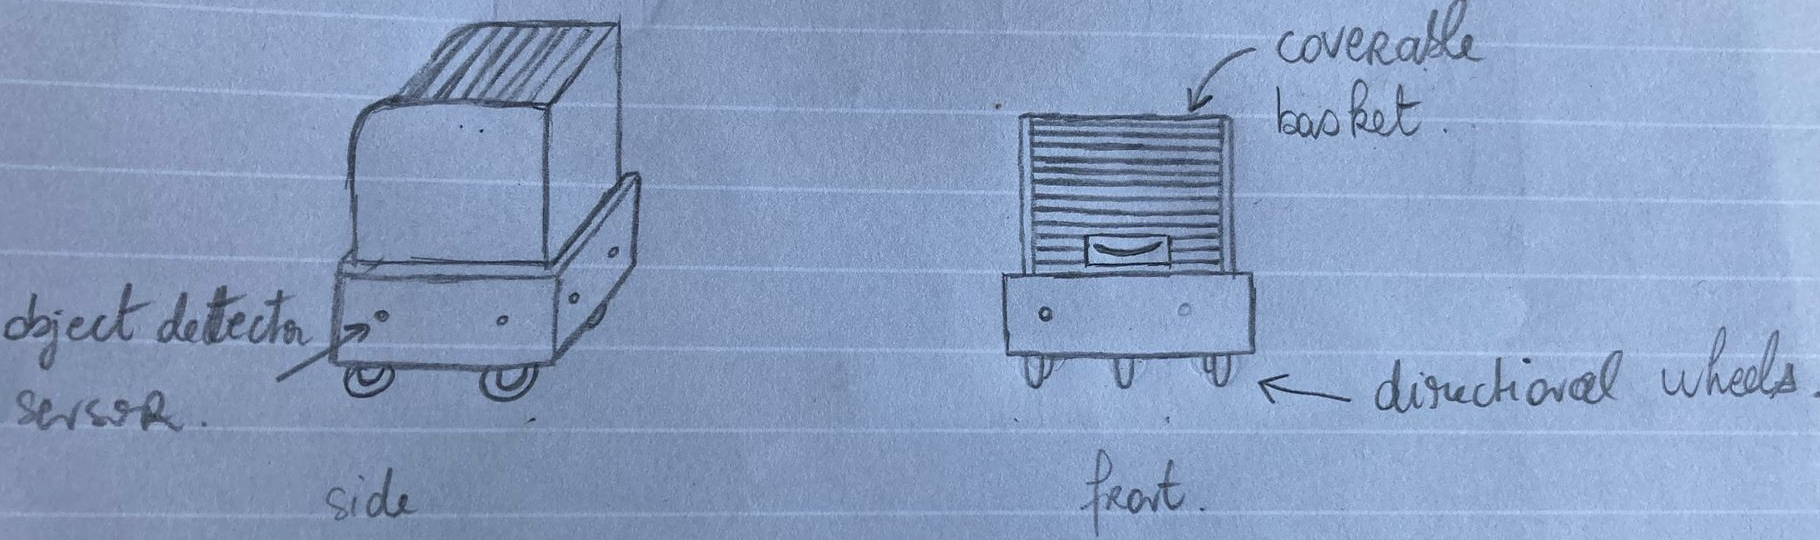
\includegraphics[scale = 0.2]{IMGs/CONCEPT1}	
	\end{subfigure}%
	\begin{subfigure}{0.5\textwidth}
		\centering	
		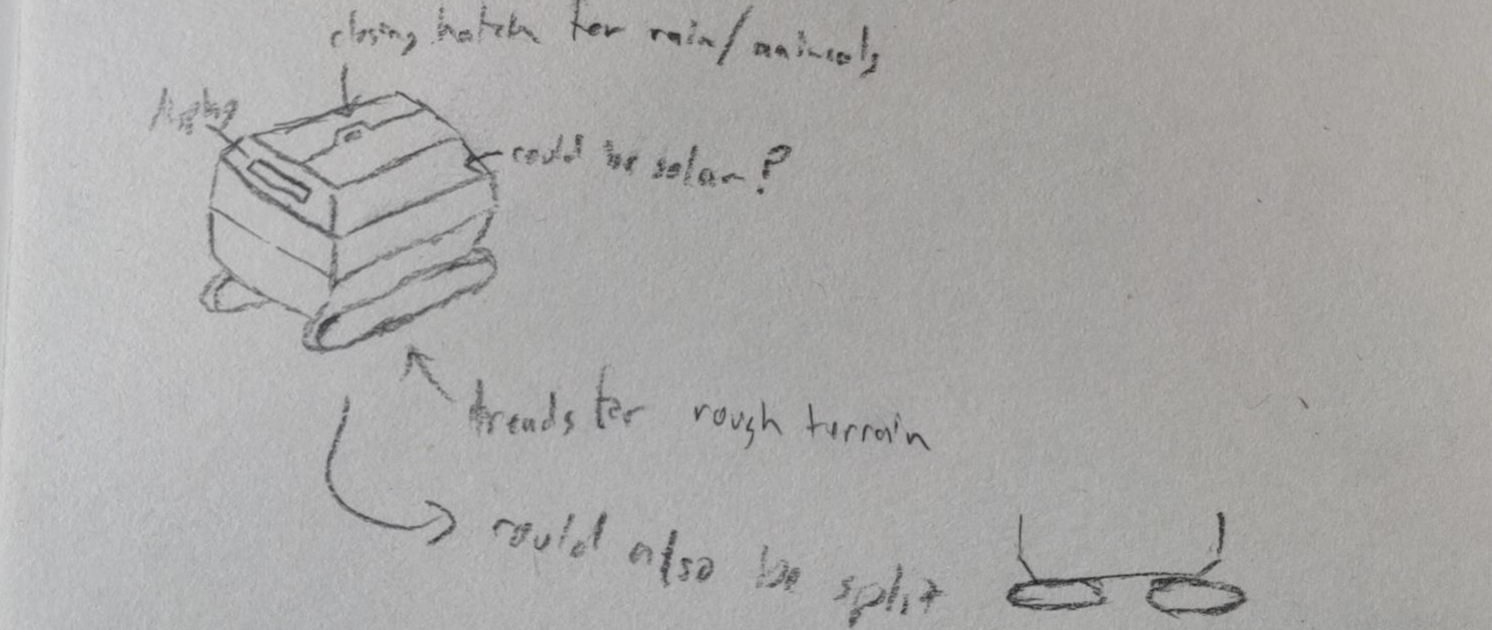
\includegraphics[scale = 0.3]{IMGs/CONCEPT2}
	\end{subfigure}
	\caption{First concept}
\end{figure}

Notice both concepts describe a robot fitted with a lid. This is not a critical function. However, it will be implemented if all the main functions of the robot are completed.

\newpage

\section{Project Tasks}

In order to work properly, we need to define small and simple steps. At every step the robot will be improved with more feature set. By the en of the project we should come up with all the main functions we defined earlier.\\
The project is divided in 3 main steps and 1 step for additional and not mandatory features :

\subsection{Proto V1: Driving (by October 26)}
Design for the electronics and casing complete. Bot prototype can drive smoothly from one coordinate to another. 

Design is finished and has been tested with 3D printing. Discuss ways to create the final prototype (3D print, CNC, Other). 

Bot has motor function and can be driven precisely to given coordinates. 

\subsection{Proto V2: Following (by November 18)}

Aim: Bot and remote can communicate causing the bot to “follow" the remote 

Remote can communicate reliably with the bot and control the bot’s path. 

GPS modules in the bot and remote act reliably. 

Bot follows the remote with a set buffer distance.  

\subsection{Proto V3: Collision (by November 23)}

Aim: Bot can sense obstacles in its path and stop to avoid them. When obstacles are removed, the bot continues. 

Bot uses necessary sensors to avoid obstacles in its path and avoid “active collisions”. 

\subsection{Proto V4: Intelligence (by December 1 (If there is time))}

Aim: Bot can understand basic situations involving obstacles and can resolve them using given information. If the issue cannot be resolved, the bot remains where it is. 

Bot can make smart decisions regarding the navigation around obstacles in order to fulfil the minimum distance from the target (remote). 